\documentclass[10pt]{beamer}
\usepackage[utf8]{inputenc}
\usepackage[spanish]{babel}
\usepackage{amsmath}
\usepackage{amsfonts}
\usepackage{amssymb}
\usepackage{graphicx}
\usepackage{lipsum}
\usepackage{ragged2e}
\usepackage{hyperref}
\usepackage{float}
\usepackage{tikz}
\usepackage{url}

% Cargar bibliotecas TikZ necesarias sin bayesnet
\usetikzlibrary{shapes.geometric, arrows, positioning, fit}

\usetheme{Madrid}
\newcommand{\celda}[1]{
	\begin{minipage}{2.5cm}
		\vspace{5mm}
		#1
		\vspace{5mm}
	\end{minipage}
}

\author[Aarón F. Alberca]{Aarón Flores Alberca}
\title[Navegación autónoma: SLAM]{Introducción a la teoría de la navegación autónoma}
\date{\today} 
\subtitle{Explicación e implementación de algoritmos SLAM con optimización gráfica}
\institute[UNI]{
	Universidad Nacional de Ingeniería. Facultad de Ciencias. \\Escuela Profesional de Ciencia de la Computación
}

\AtBeginSection[]
{
	\begin{frame}<beamer>{Contenido}
		\tableofcontents[currentsection,currentsubsection]
	\end{frame}
}

\tikzset{
    startstop/.style = {rectangle, rounded corners, minimum width=1.5cm, minimum height=0.5cm,text centered, draw=black, fill=red!30},
    process/.style = {rectangle, minimum width=1.5cm, minimum height=0.5cm, text centered, draw=black, fill=orange!30},
    arrow/.style = {thick,->,>=stealth},
    factor/.style={draw, fill=black, circle, inner sep=1.5pt},
    variable/.style={draw, fill=white, circle, minimum size=1cm},
    cloud/.style={draw, ellipse, fill=white, minimum height=2em}
}

\begin{document}
	
	\begin{frame}
		\maketitle
	\end{frame}

	\begin{frame}{Contenido}
		\tableofcontents
	\end{frame}
	
	\section{Introducción}
		\begin{frame}{Introducción}
			Se entiende a la navegación autónoma como la capacidad de un sistema, generalmente un vehículo o robot, para desplazarse sin intervención humana en un entorno ya sea conocido o desconocido.
            Para alcanzar dicha independencia se tienen dos opciones:
            \begin{itemize}
                \item \textbf{Heurísticas matématicas:}
                Se designa un conjunto de reglas generales y preestablecidas de interacción entre el móvil y su entorno para la completitud de ciertas metas.
                \item \textbf{Optimización:} 
                El agente o sistema involucrado se adecúa a su entorno capturando e interprentado datos de este para la completitud de sus tareas designadas, por lo mismo requiere de muchísima información.
            \end{itemize}
		\end{frame}

        \begin{frame}{Introducción (cont.)}
            Aunque la tarea de construir dichos modelos sea demasiado compleja, muchísimas compañías actuales se encuentran interesados en construir vehículos con dichas capacidades como Tesla, Google e incluso Nvidia.

            Se puede estructurar el funcionamiento de sistemas autónomos como el siguiente bucle:

            \begin{center}
                \begin{tikzpicture}[node distance=2.4cm]
                    % Nodos
                    \node (n1) [startstop] {Mundo físico};
                    \node (n2) [process, right of=n1] {Percibir};
                    \node (n3) [process, right of=n2] {Interpretar};
                    \node (n4) [process, below of=n3] {Planificar};
                    \node (n5) [process, left of=n4] {Actuar};
    
                    %Flechas
                    \draw [arrow] (n1) -- (n2);
                    \draw [arrow] (n2) -- (n3);
                    \draw [arrow] (n3) -- (n4);
                    \draw [arrow] (n4) -- (n5);
                    \draw [arrow] (n5) -| (n1);
                \end{tikzpicture}
            \end{center}
            
            Un componente fundamental de este ciclo es la interpretación del entorno, que implica la localización del robot y el mapeo del entorno.
        \end{frame}
        
        \begin{frame}{Sensores en navegación autónoma}
            Los robots autónomos utilizan diversos sensores para percibir el entorno:
            \begin{itemize}
            \item \textbf{LiDAR (Light Detection and Ranging):} Emite pulsos láser que rebotan en superficies y regresan, permitiendo medir distancias con precisión y crear mapas 3D del entorno.
            \item \textbf{IMU (Unidad de Medición Inercial):} Combina acelerómetros, giroscopios y magnetómetros para medir aceleración lineal y velocidad angular, proporcionando información sobre el movimiento del robot.
            \item \textbf{Cámaras:} Proporcionan información visual del entorno, utilizadas para detección de objetos, líneas y características distintivas.
            \item \textbf{Encoders:} Miden el desplazamiento de las ruedas, permitiendo estimar el movimiento del robot (odometría).
            \end{itemize}
            La fusión de estos datos sensoriales permite construir una representación coherente del entorno y de la posición del robot mediante una técnica de estimación de posición 
            que calcula el movimiento realizado llamado \textbf{odometría}.\\
            Sin embargo, la odometría acumula errores con el tiempo debido a deslizamientos, imperfecciones en las ruedas y superficies irregulares.
            \end{frame}

        \begin{frame}{El problema SLAM}
            \textbf{SLAM} (Simultaneous Localization and Mapping) es uno de los problemas fundamentales en robótica móvil.
            
            \begin{itemize}
                \item \textbf{Problema:} Un robot explora un entorno desconocido, debe construir un mapa y, simultáneamente, localizarse dentro de él.
                
                \item \textbf{Desafío:} Para construir un mapa preciso se necesita conocer la posición del robot, pero para conocer la posición se necesita un mapa fiable.
                
                \item \textbf{Incertidumbre:} Tanto el mapa como la posición del robot contienen errores que se propagan y acumulan.
            \end{itemize}
            
            \begin{center}
                \begin{tikzpicture}[scale=0.8]
                    % Robot path
                    \draw[thick, ->] (0,0) to[out=45,in=180] (2,1) to[out=0,in=135] (4,0) to[out=-45,in=180] (6,-1);
                    
                    % Robot positions
                    \node[draw, circle, fill=blue!20, minimum size=0.5cm] at (0,0) {};
                    \node[draw, circle, fill=blue!20, minimum size=0.5cm] at (2,1) {};
                    \node[draw, circle, fill=blue!20, minimum size=0.5cm] at (4,0) {};
                    \node[draw, circle, fill=blue!20, minimum size=0.5cm] at (6,-1) {};
                    
                    % Landmarks - usando shapes.geometric para estrella
                    \node[draw, regular polygon, regular polygon sides=5, fill=yellow!40, minimum size=0.5cm] at (1,2) {};
                    \node[draw, regular polygon, regular polygon sides=5, fill=yellow!40, minimum size=0.5cm] at (3,2) {};
                    \node[draw, regular polygon, regular polygon sides=5, fill=yellow!40, minimum size=0.5cm] at (5,1) {};
                    
                    % Observations
                    \draw[dashed] (0,0) -- (1,2);
                    \draw[dashed] (2,1) -- (1,2);
                    \draw[dashed] (2,1) -- (3,2);
                    \draw[dashed] (4,0) -- (3,2);
                    \draw[dashed] (4,0) -- (5,1);
                    \draw[dashed] (6,-1) -- (5,1);
                    
                    % Labels
                    \node at (0,-0.5) {\tiny Pose 1};
                    \node at (2,0.5) {\tiny Pose 2};
                    \node at (4,-0.5) {\tiny Pose 3};
                    \node at (6,-1.5) {\tiny Pose 4};
                    \node at (1,2.5) {\tiny Landmark 1};
                    \node at (3,2.5) {\tiny Landmark 2};
                    \node at (5,1.5) {\tiny Landmark 3};
                \end{tikzpicture}
            \end{center}
        \end{frame}
        
        \begin{frame}{Matrices de Transformación en Navegación Autónoma}
            \begin{itemize}
                \item \textbf{Transformación Rígida en 3D:} Representada mediante matrices $4 \times 4$ en $SE(3)$
                \begin{equation*}
                T = \begin{bmatrix} 
                R & t \\
                0_{1 \times 3} & 1
                \end{bmatrix}
                \end{equation*}
                donde $R \in SO(3)$ es la matriz de rotación y $t \in \mathbb{R}^3$ es el vector de traslación
                
                \item \textbf{Composición de transformaciones:} Multiplicación matricial
                \begin{equation*}
                T_{AB} \cdot T_{BC} = T_{AC}
                \end{equation*}
                
                \item \textbf{Transformación inversa:}
                \begin{equation*}
                T^{-1} = \begin{bmatrix} 
                R^T & -R^Tt \\
                0_{1 \times 3} & 1
                \end{bmatrix}
                \end{equation*}
            \end{itemize}
            
            \begin{center}
                \begin{tikzpicture}[scale=0.7]

                    \draw[-latex,red,thick] (0,0) -- (1.5,0) node[right] {$x_A$};
                    \draw[-latex,red,thick] (0,0) -- (0,1.5) node[above] {$y_A$};
                    \draw[-latex,red,thick] (0,0) -- (0.5,0.5,0.5) node[above] {$z_A$};
                    
                    \draw[-latex,blue,thick] (3,2) -- (4,2.8) node[right] {$x_B$};
                    \draw[-latex,blue,thick] (3,2) -- (2.2,3) node[above] {$y_B$};
                    \draw[-latex,blue,thick] (3,2) -- (3.5,2.5,0.5) node[above] {$z_B$};
                    
                    \draw[-stealth, thick, dashed] (0.8,0.7) to[bend left] node[midway, above] {$T_{AB}$} (2.5,1.8);
                \end{tikzpicture}
            \end{center}
        \end{frame}


        \begin{frame}{El algoritmo ICP}
            El algoritmo \textbf{ICP (Iterative Closest Point)} es fundamental en SLAM para alinear nubes de puntos y estimar el movimiento del robot:
            
            \begin{itemize}
                \item \textbf{Objetivo:} Encontrar la transformación (rotación y traslación) que mejor alinea dos conjuntos de puntos.
                
                \item \textbf{Proceso iterativo:}
                \begin{enumerate}
                    \item Asociar puntos entre ambas nubes (correspondencia)
                    \item Estimar la transformación que minimiza la distancia entre puntos correspondientes
                    \item Aplicar la transformación y repetir hasta converger
                \end{enumerate}
                
                \item \textbf{Aplicaciones:} Registro de scans LiDAR consecutivos, construcción de mapas 3D, estimación de odometría.
            \end{itemize}
            
            ICP es susceptible a mínimos locales, por lo que requiere una buena inicialización. Es comúnmente utilizado en combinación con otros métodos de estimación de movimiento.
        \end{frame}
	
	\section{Marco teórico}
		\begin{frame}{Conceptos de cálculo de probabilidades}
            Se denomina \textbf{variable aleatoria} (v.a) $X$ a una función real que asigna un valor numérico a resultados posibles de eventos aleatorios, matemáticamente $X$ se define como una función $X:\Omega \rightarrow E \subset\mathbf{R}$ donde $\Omega$ es un espacio muestral que determina todos los posibles valores que puede tomar dicha variable $X$ y $E \subset \mathbf{R}$ como la representación cuantificada de dichos valores aleatorios.

            De este concepto podemos tomar dos acercamientos diferentes referentes a variables aleatorias:
            \begin{itemize}
                \item \textbf{V.A discretas:} Se dice que una v.a es discreta si toma valores en un conjunto numerable (finito o infinito numerable). Ejemplo: Número de caras al lanzar 3 veces una moneda o cantidad de turistas visitantes a un museo.
                \item \textbf{V.A continuas:} Se dice que una v.a es continua si puede tomar cualquier valor dentro de un intervalo de números reales. Ejemplo: Medición de la presión en diferentes camaras de un submarino o la estimación del movimiento de un móvil mediante sensores.
            \end{itemize}
		\end{frame}

        \begin{frame}{Conceptos de cálculo de probabilidades (cont.)}
            Para esta presentación nos concentraremos en específico con las v.a continuas, con ellas podemos encontrarnos con los siguientes conceptos:
            \begin{itemize}
                \item \textbf{Función de densidad de probabilidad:} En el contexto de SLAM, la PDF más común es la distribución Gaussiana multivariada:
                
                \[
                \mathcal{N}(x; \mu, \Sigma) = p(x) = \frac{1}{\sqrt{|2\pi\Sigma|}} \exp\left(-\frac{1}{2}\|x - \mu\|^2_{\Sigma}\right)
                \]
                
                donde $\mu$ es el vector de medias, $\Sigma$ es la matriz de covarianza y $\|x - \mu\|^2_{\Sigma}$ representa la distancia de Mahalanobis de los valores $x$ con respecto a la distribución de probabilidad.

                \item \textbf{Modelación de medición}: Es conveniente el modelamiento de las mediciones hechas con incertidumbres con un ruido de tipo Gausiano de media cero y matriz de covarianza $R$. Definimos
                dicho estimación como un valor $z$:
                
                \[
                z = h(x,l) + \eta
                \]
                
                donde $h(.)$ se le denomina una función de predicción de medidad y el ruido $\eta$ el modelo de incertidumbre declarado anteriormente.
            \end{itemize}
        \end{frame}

        \begin{frame}{Conceptos de cálculo de probabilidades (cont.)}
            Es de estas inferencias de donde se llega a la siguiente función de probabilidad condicional adecuada para la medición estimada $z$:
            \[
            \mathcal{N}(z; h(x, l), R) = p(z | x, l) = \frac{1}{\sqrt{|2\pi R|}} \exp\left(-\frac{1}{2}\|h(x,l) - z\|^2_{R}\right)
            \]

            En un modelo probabilístico de movimiento, $g(.)$ representa nuestra función de predicción, $u_t$ es una acción conocida de movimiento y $Q$ es su matriz de covarianza asociada. Estos elementos conforman nuestra función de probabilidad.        
            \[
            \mathcal{N}(x_{t+1}; g(x_t, u_t), Q) = p(x_{t+1} | x_t, u_t) = \frac{1}{\sqrt{|2\pi Q|}} \exp\left(-\frac{1}{2}\|g(x_t, u_t) - x_{t+1}\|^2_{Q}\right)
            \]

            Nos topamos con un problema importante, ya que ambas probabilidades fundamentales están siendo expresadas mediante funciones de densidad diferentes aunque iguales en esencia. De estas complicaciones, introducimos
            el concepto de un factor graph como modelo gráfico probabilístico para la resolución de estas estimaciones.
        \end{frame}

        \begin{frame}{Factor Graphs}
            Un factor graph es un grafo bipartito $F = (U, V, E)$ con:
                \begin{itemize}
                    \item Nodos variables $\theta_j \in V$ (poses del robot, landmarks)
                    \item Nodos factores $\phi_i \in U$ (mediciones, restricciones)
                    \item Aristas $e_{ij} \in E$ que conectan factores con las variables de las que dependen
                \end{itemize}
                \vspace{0.2 cm}

            A partir de dicho modelo gráfico se obtiene la función de probabilidad total como la productoria de todos los nodos factores.
                $$\phi(X) = \prod_i \phi_i(X_i)$$
            donde $X_i$ son las variables conectadas al factor $\phi_i$.
            
            
            \begin{center}
                \begin{tikzpicture}
                    % Variables
                    \node[variable] (x1) at (0,0) {$x_1$};
                    \node[variable] (x2) at (2,0) {$x_2$};
                    \node[variable] (x3) at (4,0) {$x_3$};
                    \node[variable] (l1) at (1,2) {$l_1$};
                    \node[variable] (l2) at (3,2) {$l_2$};
                    
                    % Factors
                    \node[factor] (f1) at (1,0) {};
                    \node[factor] (f2) at (3,0) {};
                    \node[factor] (f3) at (0,-1) {};
                    \node[factor] (f4) at (1,1) {};
                    \node[factor] (f5) at (2,1) {};
                    \node[factor] (f6) at (3,1) {};
                    
                    % Edges
                    \draw (x1) -- (f1) -- (x2) -- (f2) -- (x3);
                    \draw (x1) -- (f3);
                    \draw (x1) -- (f4) -- (l1);
                    \draw (x2) -- (f5) -- (l1);
                    \draw (x3) -- (f6) -- (l2);
                \end{tikzpicture}
            \end{center}
        \end{frame}

        \begin{frame}{Factor Graphs en SLAM}
            Los factor graphs ofrecen una representación natural para el problema SLAM:
            
            \begin{itemize}
                \item \textbf{Variables ($X$):}
                Son variables aleatorias almacenadas en la memoria del móvil obtenidas de sus sensores adheridos, con los que se les permite tener una estimación del entorno y de su posición en él.
                \begin{itemize}
                    \item Poses del robot $x_1, x_2, ..., x_n$
                    \item Posiciones de landmarks $l_1, l_2, ..., l_m$
                \end{itemize}
                
                \item \textbf{Factores:} Representan restricciones probabilísticas sobre las variables mediante funciones de probabilidad para modelar características como mediciones y movimiento.
                
                \[
                \begin{aligned}
                    \phi_i(X_i) &= \frac{1}{\sqrt{|2\pi \Sigma_i|}} \exp \left\{-\frac{1}{2}\|h_i(X_i) - z_i\|^2_{\Sigma_i} \right\} \\
                    & \propto \exp \left\{-\frac{1}{2}\|h_i(X_i) - z_i\|^2_{\Sigma_i} \right\}
                \end{aligned}
                \]
            \end{itemize}
            
        \end{frame}
        
        \begin{frame}{Inferencia MAP - Máximo a posteriori}
            
            La inferencia MAP busca la configuración más probable de las variables dado los datos observados:
            
            \[
                X^{MAP} = \arg\max_{X}\phi(X) = \arg\max_{X} \prod_i \phi_i(X_i)
            \]
            
            Podemos convertir nuestra inferencia inicial de la siguiente manera:
            \[
            \begin{aligned}
                X^{MAP} &\propto \arg\max_{X} \exp \left\{ \sum_i - \frac{1}{2} \|h_i(X_i) - z_i\|^2_{\Sigma_i} \right\} \\ 
                &\propto \arg\min_{X} \sum_i \|h_i(X_i) - z_i\|^2_{\Sigma_i}
            \end{aligned}
            \]
            
            Así, la inferencia MAP se transforma en un problema de mínimos cuadrados ponderados, donde cada término representa la discrepancia entre la predicción del modelo $h_i(X_i)$ y la medición $z_i$, ponderada por la incertidumbre $\Sigma_i^{-1}$.
            

        \end{frame}

        \begin{frame}{Linearización}
            Podemos linealizar nuestras funciones de medición $h_i(.)$ dentro de una simple expansión de una serie de Taylor como la siguiente:
            \[
            h_i(X_i) = h_i(X^0_i + \Delta_i) \approx h_i(X^0_i) + H_i \Delta_i
            \]
            Donde $X^0_i$ es un estado inicial de nuestras estimaciones de valores $X_i$, $\Delta_i$ es la diferencia entre dicho estado inicial y el estado a evaluar $X_i - X^0_i$ y finalmente adaptamos a un jacobiano de medición como $H_i$ con la siguiente definición:
            \[
            H_i = \left.\frac{\partial h_i(X_i)}{\partial X_i}\right|_{X_i^0}
            \]

            Substituimos nuestra aproximación realizada dentro de nuestra anterior conceptualización de MAP para cambiar nuestro enfoque de variables que maximizan a un vector de cambio que maximiza:
            \[
            \begin{aligned}
                \Delta^* &= \arg\min_\Delta \sum_i \|h_i(X^0_i) + H_i\Delta_i - z_i \|^2_{\Sigma_i} \\
                &=  \arg\min_\Delta \sum_i \|H_i\Delta_i - \left\{z_i - h_i(X^0_i)\right\} \|^2_{\Sigma_i} 
            \end{aligned}
            \]
        \end{frame}

        \begin{frame}{Linearización (cont.)}
            Nos encontramos sometidos a una distancia de Mahalanobis, lo que no permite un desarrollo computacionalmente simple, para esto recordemos que
            nuestra matriz de covarianza es una matriz semidefinida positiva con lo cual se nos permite encontrar una matriz raíz cuadrada a partir de algún método de factorización como LU.
            \[
            \|e\|^2_\Sigma = e^T \Sigma^{-1} e = \left(\Sigma^{-1/2}e\right)^T \left(\Sigma^{-1/2}e\right) = \|\Sigma^{-1/2} e\|^2_2
            \]

            Si considerasemos a nuestro error $e = H_i\Delta_i - \left\{z_i - h_i(X^0_i)\right\}$ entonces llegamos a los siguientes conceptos:
            \[
            \begin{aligned}
                A_i &= \Sigma^{-1/2}_i H_i \\
                b_i &= \Sigma^{-1/2}_i \left(z_i - h_i(X^0_i)\right)
            \end{aligned}
            \]

            Reemplazándolo en nuestra problemática inicial nos daremos cuenta de algo interesante:
            \[
                \begin{aligned}
                    \Delta^* &= \arg\min_\Delta \sum_i \|A_i \Delta_i - b_i \|^2_2 \\
                    &=  \arg\min_\Delta \|A \Delta - b \|^2_2 
                \end{aligned}
            \]

            Llegamos a un sistema de ecuaciones lineales

        \end{frame}
        
        \begin{frame}{Método del descenso de gradiente}
            Con esta nueva conversión podemos encontrarnos con distintos métodos de resolución que serían una factorización QR, 
            Gauss-Newton, Levenberg-Marquardt, etc. Abarcaremos el más 'simple' mediante el descenso de gradiente.
            \vspace{0.3 cm}

            Damos el siguiente modelo iterativo para encontrar una solución a nuestro problema:
            \[
            X^{t+1} = X^t + \Delta
            \]

            Comenzamos definiendo a nuestra función costo como la siguiente:
            \[
            g(X) = \sum_i \|h_i(X_i) - z_i\|^2_{\Sigma_i} \approx \|A(X - X^t) - b\|^2_2
            \]
            
            Finalmente calculamos a $\Delta$ mediante esta aproximación:
            \[
            \Delta = - \alpha \nabla \left. g(X) \right|_{X = X^t} = - \alpha \left(-2 A^T b\right) = 2 \alpha A^Tb 
            \]
            
            \[
            X^{t+1} = X^t + 2 \alpha A^Tb 
            \]

            donde $\alpha$ es la tasa de convergencia, lamentablemente se vuelve ligeramente lento al encontrar mínimos.
        \end{frame}

        \section{Explotando la Dispersión}
        \begin{frame}{Estructura Dispersa en SLAM}
            La dispersión es una característica fundamental en SLAM que refleja la naturaleza física de las mediciones robóticas:
            En problemas SLAM, la matriz inicial $A$ y la de información $\Lambda = A^T A$ presenta una alta dispersión debido a las siguientes razones:
            \begin{itemize}
                \item Cada medición relaciona solo unas pocas variables (generalmente solo dos)
                \item Poses consecutivas del robot están conectadas formando una cadena
                \item Los landmarks solo son observados desde un pequeño subconjunto de poses
            \end{itemize}
                
            En la siguiente matriz podemos encontrarnos con la representación del sistema de ecuaciones lineales de nuestro ejemplo inicial:
            
            \begin{figure}
                \centering
                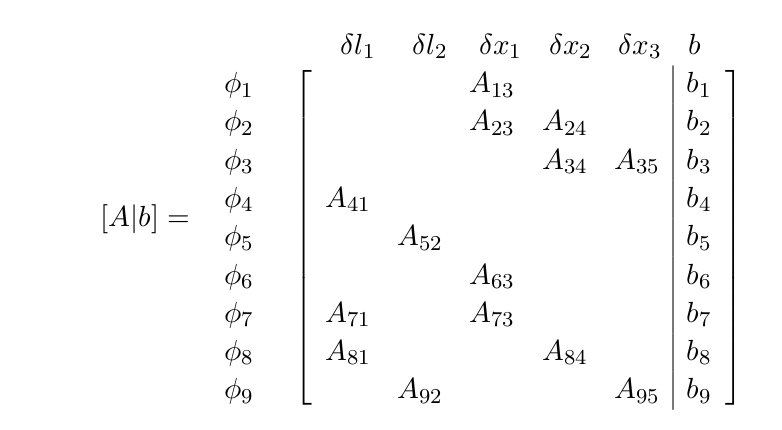
\includegraphics[width=0.5\linewidth]{matrix sparse.png}
            \end{figure}
            
            El reconocimiento y explotación de esta dispersión permite transformar problemas aparentemente intratables en computacionalmente viables.
        \end{frame}
        
        \begin{frame}{Beneficios Computacionales de la Dispersión}
            Esta estructura dispersa tiene un impacto directo en la representación computacional:
            
            \begin{itemize}
                \item \textbf{Eficiencia en almacenamiento:} Solo se almacenan los elementos no-cero mediante formatos especializados como CSR o CSC, reduciendo el consumo de memoria en más del 99\% para problemas grandes.
                
                \item \textbf{Operaciones matriciales optimizadas:} Las operaciones básicas se vuelven significativamente más eficientes.
                \begin{itemize}
                    \item Multiplicación matriz-vector: $O(k)$ en lugar de $O(n^2)$
                    \item Factorización de la matriz: $O(n)$ en vez de $O(n^3)$ para muchas configuraciones de SLAM
                \end{itemize}
                
                \item \textbf{Algoritmos adaptados:} Se pueden utilizar técnicas especializadas como el ordenamiento de variables, la actualización incremental y las implementaciones distribuidas y paralelas para resolver ese tipo de problemas a gran escala.
            \end{itemize}
            
            Estas ventajas permiten resolver sistemas con millones de variables, haciendo posible aplicaciones de SLAM en tiempo real y a gran escala.
        \end{frame}

        \section{Algoritmos avanzados para SLAM}
        \begin{frame}{Algoritmos de Odometría LiDAR}
            \textbf{KISS-ICP:} Simplicidad efectiva con adaptación de velocidad para predicción de movimiento, ponderación por Mahalanobis y rechazo inteligente de outliers. Destaca por su rendimiento superior con implementación de menos de 500 líneas de código. Ideal para sistemas con recursos limitados.
            
            \vspace{0.5cm}
            
            \textbf{CT-ICP:} Corrección de distorsión temporal mediante modelado de trayectoria con B-splines, desdistorsión de puntos según timestamp y adaptación del intervalo de control según velocidad. Especialmente efectivo en vehículos de alta velocidad, drones y robots ágiles donde la distorsión es significativa.
            
            \vspace{0.5cm}
            
            \textbf{GLIM:} Fusión LiDAR-IMU en factor graphs con optimización conjunta de poses y velocidades. Integra factores complementarios (LiDAR, IMU, loop closure) y calibración en línea. Proporciona robustez en entornos con poca geometría o movimiento rápido, manteniendo la consistencia global del mapa.
        \end{frame}

        \section{Conclusiones}
        \begin{frame}{Conclusiones}
            \begin{itemize}
                \item Los factor graphs proporcionan un marco unificado para representar y resolver problemas de SLAM.
                
                \item La estructura dispersa de los problemas SLAM permite algoritmos eficientes.
                
                \item La optimización no lineal sobre manifolds es clave para manejar correctamente rotaciones y transformaciones.
                
                \item Los algoritmos incrementales permiten aplicaciones en tiempo real.
                
                \item El campo continúa evolucionando hacia sistemas más robustos y aplicaciones en entornos complejos.
            \end{itemize}
            
            Los factor graphs se han convertido en el enfoque dominante para SLAM, proporcionando una base teórica sólida y soluciones prácticas para la navegación autónoma.
        \end{frame}

    \section{Referencias}
        \begin{frame}{Referencias}
            [1] Factor Graphs for Robot Perception. (s. f.). Now Foundations And Trends Books | IEEE Xplore. \url{https://ieeexplore.ieee.org/document/8187520}
            \vspace{0.3 cm}

            [2] Vizzo, I., Guadagnino, T., Mersch, B., Wiesmann, L., Behley, J., & Stachniss, C. (2023). KISS-ICP: In Defense of Point-to-Point ICP – Simple, Accurate, and Robust Registration If Done the Right Way. IEEE Robotics And Automation Letters, 8(2), 1029-1036. \url{https://doi.org/10.1109/lra.2023.3236571}
            \vspace{0.3 cm}

            [3] Dellenbach, P., Deschaud, J., Jacquet, B., & Goulette, F. (2021, 27 septiembre). CT-ICP: Real-time Elastic LiDAR Odometry with Loop Closure. arXiv.org. \url{https://arxiv.org/abs/2109.12979}
            \vspace{0.3 cm}

            [4] Koide, K., Yokozuka, M., Oishi, S., & Banno, A. (2024). GLIM: 3D range-inertial localization and mapping with GPU-accelerated scan matching factors. Robotics And Autonomous Systems, 179, 104750. \url{https://doi.org/10.1016/j.robot.2024.104750}
            \vspace{0.3 cm}

        \end{frame}
\end{document}